% !TeX program = xelatex
% Academic block diagrams for the current RV32IM/Zicsr CPU.
\documentclass[tikz,multi=tikzpicture,border=8pt]{standalone}

\usepackage{fontspec}
\setmainfont{Times New Roman}
\setsansfont{Times New Roman}
\setmonofont{Times New Roman}

\usetikzlibrary{
  arrows.meta,
  backgrounds,
  calc,
  fit,
  positioning
}

\definecolor{ink}{HTML}{26384A}
\definecolor{muted}{HTML}{607286}
\definecolor{linegray}{HTML}{AAB6C2}
\definecolor{groupfill}{HTML}{F7F9FB}
\definecolor{frontendfill}{HTML}{E8F1F7}
\definecolor{decodefill}{HTML}{EAF4ED}
\definecolor{executefill}{HTML}{F2ECF8}
\definecolor{memoryfill}{HTML}{FFF2DF}
\definecolor{writebackfill}{HTML}{E9F4F2}
\definecolor{data}{HTML}{356B9A}
\definecolor{memory}{HTML}{C77B24}
\definecolor{control}{HTML}{B84A52}
\definecolor{forward}{HTML}{76519A}

\tikzset{
  font=\rmfamily,
  outer/.style={
    draw=ink,
    rounded corners=2pt,
    line width=0.8pt,
    fill=groupfill
  },
  group/.style={
    draw=linegray,
    rounded corners=2pt,
    line width=0.65pt,
    fill=groupfill
  },
  block/.style={
    draw=ink,
    rounded corners=2pt,
    line width=0.7pt,
    fill=frontendfill,
    align=center,
    text=ink,
    minimum width=2.7cm,
    minimum height=1.15cm,
    inner sep=5pt
  },
  peripheral/.style={
    block,
    fill=memoryfill,
    minimum width=2.7cm,
    minimum height=1.50cm,
    font=\rmfamily\small
  },
  io/.style={
    draw=linegray,
    rounded corners=1.5pt,
    fill=white,
    align=center,
    text=ink,
    minimum width=2.7cm,
    minimum height=0.78cm,
    inner sep=4pt,
    font=\rmfamily\small
  },
  group label/.style={font=\rmfamily\bfseries\small, text=ink, anchor=south west},
  lane label/.style={font=\rmfamily\bfseries\scriptsize, text=ink, anchor=south west},
  datapath/.style={-{Latex[length=2.5mm,width=1.7mm]}, draw=data, line width=1.0pt},
  databoth/.style={{Latex[length=2.3mm,width=1.6mm]}-{Latex[length=2.3mm,width=1.6mm]}, draw=data, line width=1.0pt},
  mempath/.style={-{Latex[length=2.5mm,width=1.7mm]}, draw=memory, line width=1.0pt},
  memboth/.style={{Latex[length=2.3mm,width=1.6mm]}-{Latex[length=2.3mm,width=1.6mm]}, draw=memory, line width=1.0pt},
  controlpath/.style={-{Latex[length=2.4mm,width=1.7mm]}, draw=control, dashed, line width=0.9pt},
  forwardpath/.style={-{Latex[length=2.4mm,width=1.7mm]}, draw=forward, line width=0.95pt},
  bus label/.style={font=\rmfamily\scriptsize, text=muted, fill=white, inner sep=1.5pt, align=center},
  stage/.style={
    draw=ink,
    rounded corners=2pt,
    line width=0.7pt,
    align=center,
    text=ink,
    minimum width=3.05cm,
    minimum height=3.35cm,
    text width=2.72cm,
    inner sep=5pt,
    font=\rmfamily\small
  },
  pipeline register/.style={
    draw=ink,
    rounded corners=1pt,
    line width=0.7pt,
    fill=white,
    minimum width=0.56cm,
    minimum height=7.50cm,
    inner sep=1pt,
    text=ink,
    font=\rmfamily\scriptsize\bfseries
  },
  shared/.style={
    block,
    minimum width=3.4cm,
    minimum height=1.35cm,
    font=\rmfamily\small
  }
}

\begin{document}

% =============================================================================
% Dual-issue CPU microarchitecture
% =============================================================================
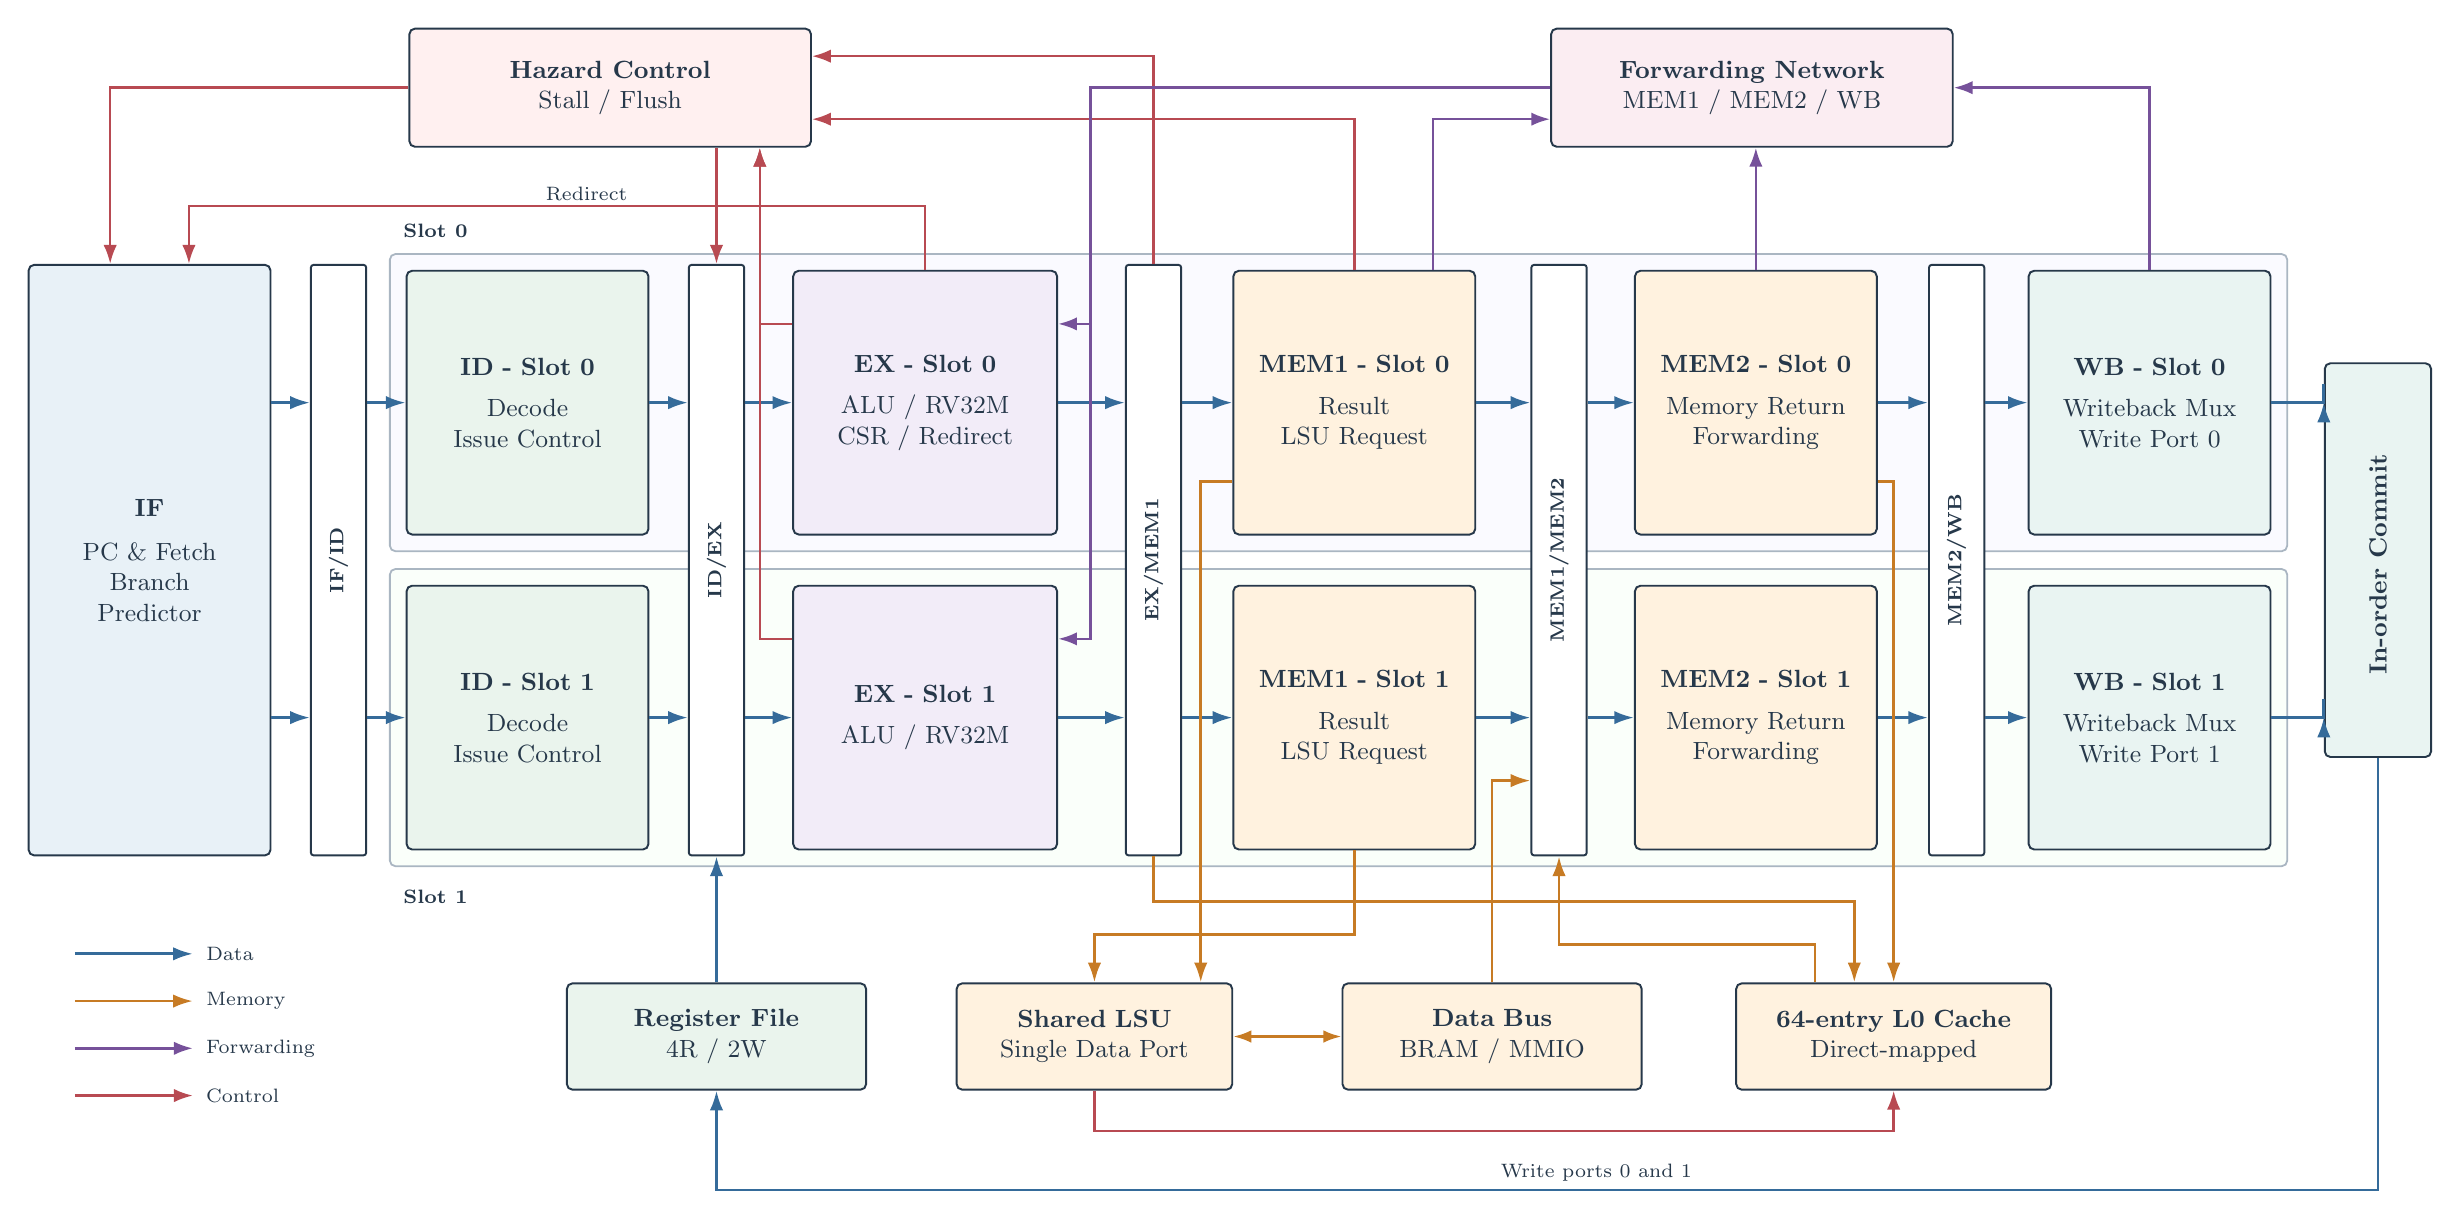
\begin{tikzpicture}[x=1cm,y=1cm]
  % Shared front end
  \node[stage, fill=frontendfill, minimum height=7.50cm] (ifstage) at (-0.55,4) {
    {\bfseries IF}\\[5pt]
    PC \& Fetch\\
    Branch\\ Predictor
  };

  % Pipeline registers
  \node[pipeline register, minimum height=20pt, minimum width=7.5cm, rotate=90] (ifid) at (1.85,4) {IF/ID};
  \node[pipeline register, minimum height=20pt, minimum width=7.5cm, rotate=90] (idex) at (6.65,4) {ID/EX};
  \node[pipeline register, minimum height=20pt, minimum width=7.5cm, rotate=90] (exmem) at (12.2,4) {EX/MEM1};
  \node[pipeline register, minimum height=20pt, minimum width=7.5cm, rotate=90] (mem1mem2) at (17.35,4) {MEM1/MEM2};
  \node[pipeline register, minimum height=20pt, minimum width=7.5cm, rotate=90] (mem2wb) at (22.4,4) {MEM2/WB};

  % Slot 0
  \node[stage, fill=decodefill] (id0) at (4.25,6) {
    {\bfseries ID - Slot 0}\\[4pt]
    Decode\\
    Issue Control
  };
  \node[stage, fill=executefill, minimum width=3.35cm, text width=3.0cm] (ex0) at (9.3,6) {
    {\bfseries EX - Slot 0}\\[4pt]
    ALU / RV32M\\
    CSR / Redirect
  };
  \node[stage, fill=memoryfill] (mem10) at (14.75,6) {
    {\bfseries MEM1 - Slot 0}\\[4pt]
    Result\\
    LSU Request
  };
  \node[stage, fill=memoryfill] (mem20) at (19.85,6) {
    {\bfseries MEM2 - Slot 0}\\[4pt]
    Memory Return\\
    Forwarding
  };
  \node[stage, fill=writebackfill] (wb0) at (24.85,6) {
    {\bfseries WB - Slot 0}\\[4pt]
    Writeback Mux\\
    Write Port 0
  };

  % Slot 1
  \node[stage, fill=decodefill] (id1) at (4.25,2) {
    {\bfseries ID - Slot 1}\\[4pt]
    Decode\\
    Issue Control
  };
  \node[stage, fill=executefill, minimum width=3.35cm, text width=3.0cm] (ex1) at (9.3,2) {
    {\bfseries EX - Slot 1}\\[4pt]
    ALU / RV32M
  };
  \node[stage, fill=memoryfill] (mem11) at (14.75,2) {
    {\bfseries MEM1 - Slot 1}\\[4pt]
    Result\\
    LSU Request
  };
  \node[stage, fill=memoryfill] (mem21) at (19.85,2) {
    {\bfseries MEM2 - Slot 1}\\[4pt]
    Memory Return\\
    Forwarding
  };
  \node[stage, fill=writebackfill] (wb1) at (24.85,2) {
    {\bfseries WB - Slot 1}\\[4pt]
    Writeback Mux\\
    Write Port 1
  };

  \begin{scope}[on background layer]
    \node[group, fill=blue!2, fit=(id0)(ex0)(mem10)(mem20)(wb0),
          inner xsep=0.20cm, inner ysep=0.20cm] (lane0box) {};
    \node[group, fill=green!2, fit=(id1)(ex1)(mem11)(mem21)(wb1),
          inner xsep=0.20cm, inner ysep=0.20cm] (lane1box) {};
  \end{scope}
  \node[lane label] at ($(lane0box.north west)+(0.06,0.08)$) {Slot 0};
  \node[lane label] at ($(lane1box.south west)+(0.06,-0.58)$) {Slot 1};

  % Main pipeline data paths
  \draw[datapath] ($(ifstage.east)+(0,2.00)$) -- (ifid.north |- id0.west);
  \draw[datapath] ($(ifstage.east)+(0,-2.00)$) -- (ifid.north |- id1.west);
  \draw[datapath] (ifid.south |- id0.west) -- (id0.west);
  \draw[datapath] (ifid.south |- id1.west) -- (id1.west);
  \draw[datapath] (id0.east) -- (idex.north |- id0.east);
  \draw[datapath] (id1.east) -- (idex.north |- id1.east);
  \draw[datapath] (idex.south |- ex0.west) -- (ex0.west);
  \draw[datapath] (idex.south |- ex1.west) -- (ex1.west);
  \draw[datapath] (ex0.east) -- (exmem.north |- ex0.east);
  \draw[datapath] (ex1.east) -- (exmem.north |- ex1.east);
  \draw[datapath] (exmem.south |- mem10.west) -- (mem10.west);
  \draw[datapath] (exmem.south |- mem11.west) -- (mem11.west);
  \draw[datapath] (mem10.east) -- (mem1mem2.north |- mem10.east);
  \draw[datapath] (mem11.east) -- (mem1mem2.north |- mem11.east);
  \draw[datapath] (mem1mem2.south |- mem20.west) -- (mem20.west);
  \draw[datapath] (mem1mem2.south |- mem21.west) -- (mem21.west);
  \draw[datapath] (mem20.east) -- (mem2wb.north |- mem20.east);
  \draw[datapath] (mem21.east) -- (mem2wb.north |- mem21.east);
  \draw[datapath] (mem2wb.south |- wb0.west) -- (wb0.west);
  \draw[datapath] (mem2wb.south |- wb1.west) -- (wb1.west);

  % Register file and in-order commit
  \node[shared, fill=decodefill, minimum width=3.8cm] (regfile) at (6.65,-2.05) {
    {\bfseries Register File}\\4R / 2W
  };
  \draw[datapath] (regfile.north) -- (idex.west);

  \node[shared, fill=writebackfill, minimum width=5cm, rotate=90] (commit) at (27.75,4) {
    {\bfseries In-order Commit}
  };
  \draw[datapath] (wb0.east) -| (wb0.east -| commit.north);
  \draw[datapath] (wb1.east) -| (wb1.east -| commit.north);
  \draw[datapath] (commit.west) |- (24.65,-4) -- node[bus label, above=1pt, fill=none, text=ink] {Write ports 0 and 1} (11,-4) -| (regfile.south);

  % Hazard, stall, flush, and redirect control
  \node[shared, fill=red!6, minimum width=5.1cm, minimum height=1.50cm] (hazard) at (5.30,10.00) {
    {\bfseries Hazard Control}\\Stall / Flush
  };
  \draw[controlpath, solid] (exmem.east) |- ($(hazard.east)+(0,0.4)$);
  \draw[controlpath, solid] (mem10.north) |- ($(hazard.east)+(0,-0.4)$);
  \draw[controlpath, solid] (hazard.west) -| ($(ifstage.north)+(-0.5,0)$);
  \draw[controlpath, solid] (hazard.south -| idex.east) -| (idex.east);

  \draw[controlpath, solid] (ex0.north) |- (8.5,8.5)
    -- node[bus label, above, fill=none, text=ink] {Redirect} (1.5,8.5) -| ($(ifstage.north)+(0.5,0)$);

  \coordinate (busyjoin) at ($(hazard.south)+(1.9,0)$);
  \draw[controlpath, solid] ($(ex0.west)+(0,1)$) -| (busyjoin);
  \draw[controlpath, solid] ($(ex1.west)+(0, 1)$) -| (busyjoin);

  % Forwarding control and data selection
  \node[shared, fill=purple!7, minimum width=5.1cm, minimum height=1.50cm] (forwarding) at (19.8,10) {
    {\bfseries Forwarding Network}\\MEM1 / MEM2 / WB
  };
  \draw[forwardpath] ($(mem10.north)+(1,0)$) |- ($(forwarding.west)+(0,-0.4)$);
  \draw[forwardpath] (mem20.north) -- (mem20.north |- forwarding.south);
  \draw[forwardpath] (wb0.north) |- (forwarding.east);
  \draw[forwardpath] (forwarding.west) -| (11.4,8) |- ($(ex0.east)+(0,1)$);
  \draw[forwardpath] (forwarding.west) -| (11.4,8) |- ($(ex1.east)+(0,1)$);

  % Shared LSU, L0 cache, and data bus
  \node[shared, fill=memoryfill, minimum width=3.5cm, text width=3.05cm] (lsu) at (11.45,-2.05) {
    {\bfseries Shared LSU}\\Single Data Port
  };
  \node[shared, fill=memoryfill, minimum width=4.0cm, text width=3.55cm] (l0) at (21.6,-2.05) {
    {\bfseries 64-entry L0 Cache}\\Direct-mapped
  };
  \node[shared, fill=memoryfill, minimum width=3.8cm, text width=3.35cm] (databus) at (16.5,-2.05) {
    {\bfseries Data Bus}\\BRAM / MMIO
  };

  \draw[mempath] ($(mem10.west)+(0,-1)$) -| ($(lsu.north)+(1.35,0)$);
  \draw[mempath] (mem11.south) |- (12.09,-0.75) -| (lsu.north);
  \draw[memboth] (lsu.east) -- (databus.west);
  \draw[mempath] (databus.north) |- ($(mem1mem2.north)+(0,-2.8)$);

  \draw[mempath] (exmem.west) |- (15.5,-0.34) -| ($(l0.north)+(-0.5,0)$);
  \draw[mempath] ($(l0.north)+(-1,0)$) |-(19,-0.88) -| (mem1mem2.west);
  \draw[mempath] ($(mem20.east)+(0,-1)$) -| (l0.north);
  \draw[controlpath, solid] (lsu.south) |-(16.42,-3.25) -| (l0.south);

  % Line legend
  \draw[datapath] (-1.5,-1) -- (0,-1)
    node[bus label, right=1mm, fill=none, text=ink] {Data};
  \draw[mempath] (-1.5,-1.6) -- (0,-1.6)
    node[bus label, right=1mm, fill=none, text=ink] {Memory};
  \draw[forwardpath] (-1.5,-2.2) -- (0,-2.2)
    node[bus label, right=1mm, fill=none, text=ink] {Forwarding};
  \draw[controlpath, solid] (-1.5,-2.8) -- (0,-2.8)
    node[bus label, right=1mm, fill=none, text=ink] {Control};
\end{tikzpicture}

\end{document}
